\documentclass[12pt, a4paper]{article}
\usepackage{graphicx}
\graphicspath{ {./imgs/} }
\usepackage{float}
\usepackage{listings}
\usepackage{color}

\definecolor{codegreen}{rgb}{0,0.6,0}
\definecolor{codegray}{rgb}{0.5,0.5,0.5}
\definecolor{codeorange}{rgb}{1,0.49,0}
\definecolor{backcolour}{rgb}{0.95,0.95,0.96}

\lstset{
  backgroundcolor=\color{backcolour},   
  commentstyle=\color{codegray},
  keywordstyle=\color{codeorange},
  numberstyle=\tiny\color{codegray},
  stringstyle=\color{codegreen},
  basicstyle=\ttfamily\footnotesize,
  breakatwhitespace=false,         
  breaklines=true,                 
  captionpos=b,                    
  keepspaces=true,                 
  numbers=left,                    
  numbersep=5pt,                  
  showspaces=false,                
  showstringspaces=false,
  showtabs=false,                  
  tabsize=2,
  xleftmargin=10pt,
}
\renewcommand{\lstlistingname}{Code}

\counterwithin{figure}{section}

%to write code:
%\begin{lstlisting}[language=java, caption={my caption}]
%    
%\end{lstlisting}

%to insert an image
%\begin{figure}[H]
%  \centering
%  \includegraphics[width=\columnwidth]{img}
%  \caption{description of the image}
%\end{figure}

%\section{Task X - XXX}
%\subsection{XXX page}
%\subsubsection{XXX.jsp}
%\subsubsection{XXX.java}
%\subsubsection{Screenshots}

\title{Web Architectures - Delivery 2}
\author{Marrocco Simone}

\begin{document}
  \maketitle
  \begin{figure}[H]
    \centering
    
\includegraphics[scale=0.35]{unitn.png}
  \end{figure}
  \tableofcontents
  \pagebreak

  \section{Introduction}
  In this assignment we were asked to create a webapp to play a simple "Guess the Flag" game. We were given different tasks to code in order to make the webapp work.

  The source code can also be found on github, on \\
  https://github.com/Marrocco-Simone/servlet\_flag\_game

  \section{Task 1 - Authentication and Registration}
\subsection{The task}
The webapp requires authentication and registration to the server. Authentication should last a defined amount of time.

To do that, at the login page we verify the credentials and then create a new session where we save the username, while for the registration we first create a new set of credentials and then create a similar session.

The credentials are stored in the shared memory of the servlet context. Since it is shared, we need to synchronize the block where we use it. What we save inside it, as the attribute \textit{user} is an array of the class \textit{UserCredentials.java}, which has fields for username and password and is serializable (useful for task 9). It also uses Bean standard, meaning we need to use get and set functions to modify the fields inside (which are private).

Inside the context we also save another attribute \textit{logged}, which contains an array of the class \textit{UserSession.java}. This class contains the fields username and points, which are the same values we save inside the session we give back to the user. It will be useful later for task 8. Like \textit{UserCredentials.java}, it uses Bean standard.
\subsection{Login page}
\subsubsection{login.jsp}
The login jsp page is simple: at the start of the file, we take the \textit{error\_msg} attribute for the request, and if not null we add it in the page in a paragraph.

We also have a form for the login and a link to the Register page.
\subsubsection{Login.java}
For the login page, we have two methods, GET and POST. The GET method simply forwards the request to the \textit{login.jsp} file. For the POST method we loop through each set of credentials that we have: if we cannot find the given username or if the password is not correct, we forward back to the jsp page with an error message. The way we do that is simple: the jsp page accepts an \textit{error\_msg} attribute.

The place where we have saved the credentials of our users is in the context, so at the start of the POST method we use the function \textit{getUsersFromContext} to get all the credentials saved in our system.

If the credentials are ok, we create a new session in the \textit{setSession} function (or we change the current session, if the user went again to the login page), where we save the username and a point filed initialized at zero (as requested in the task 2). This function also modifies the context: it will be explained later, as it is another task objective.


\subsubsection{Screenshots}
\begin{figure}[H]
  \centering
  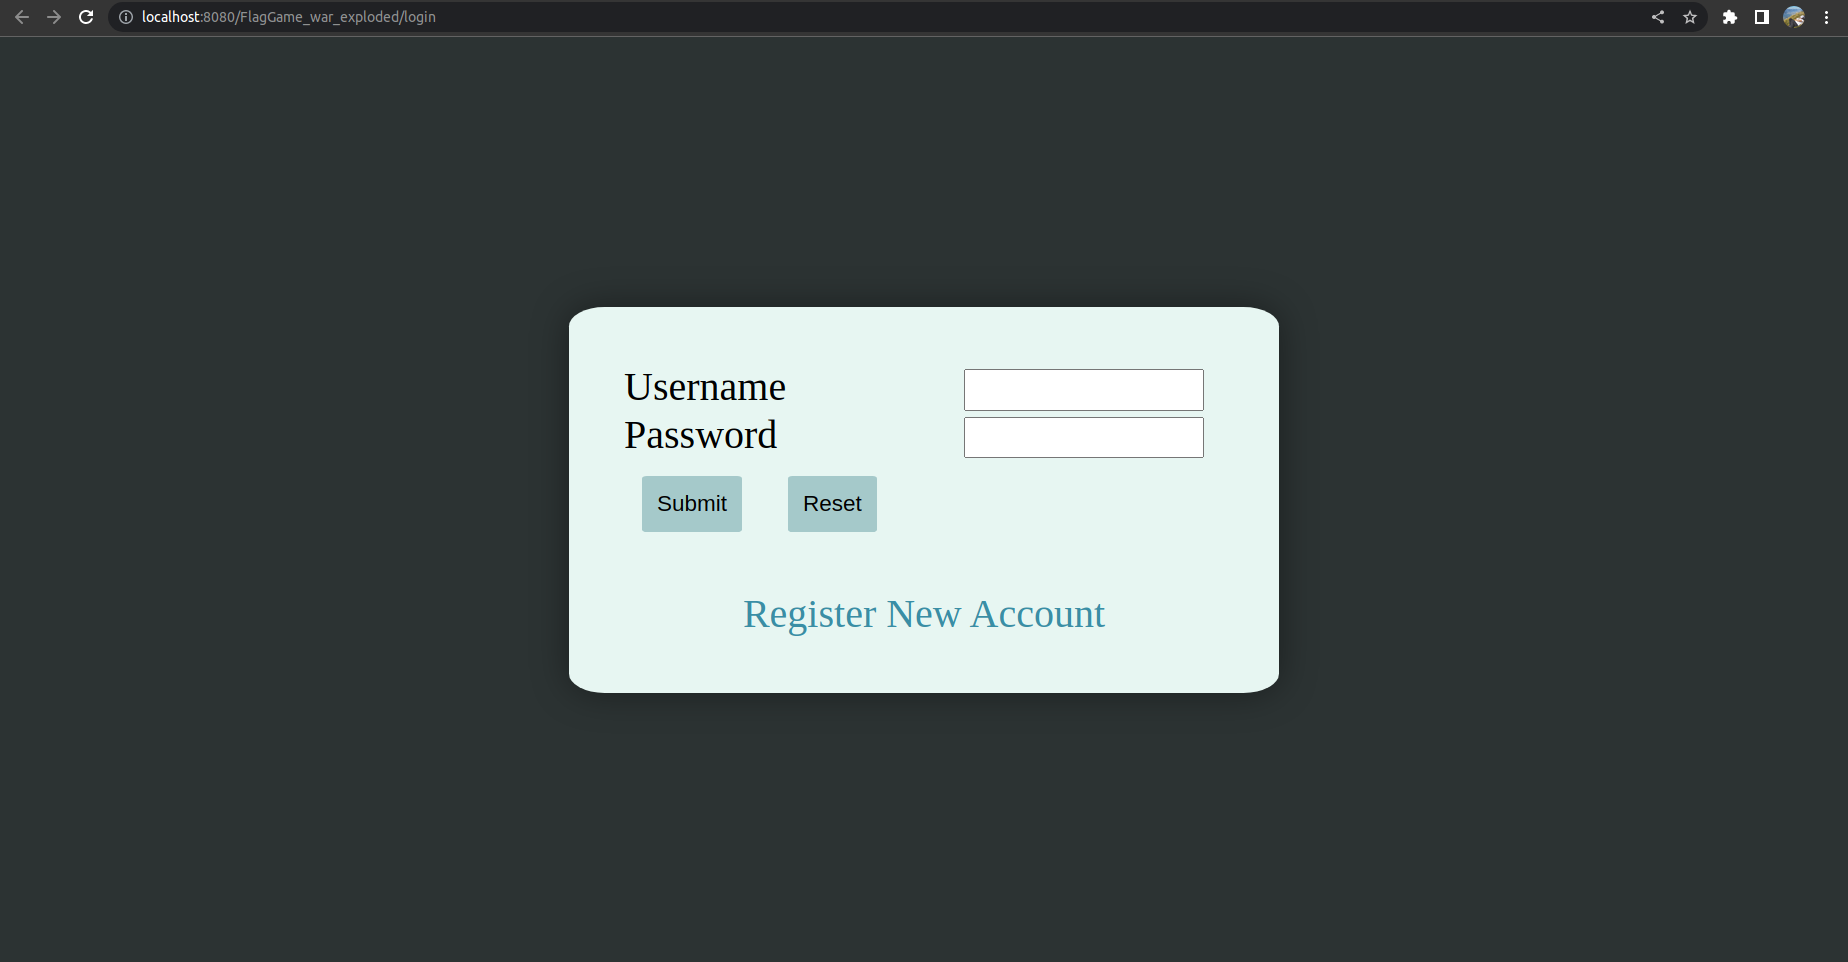
\includegraphics[width=\columnwidth]{login.png}
  \caption{Login Page}
\end{figure}
\begin{figure}[H]
  \centering
  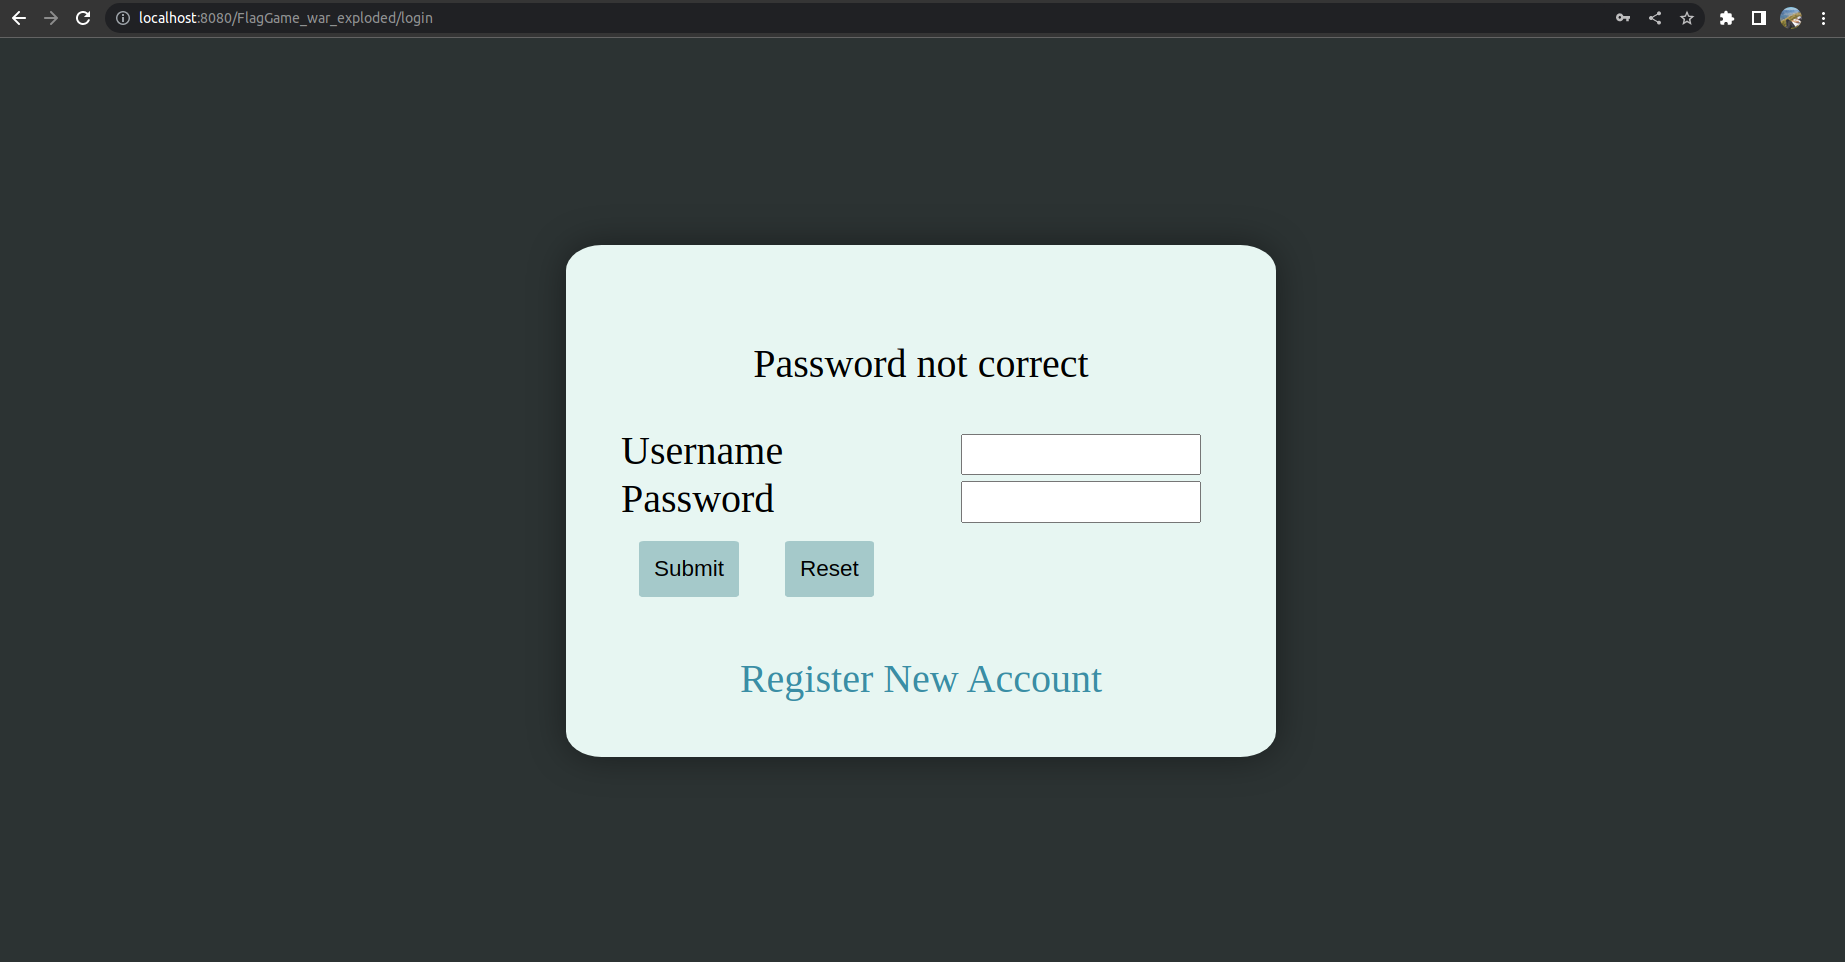
\includegraphics[width=\columnwidth]{login_password_not_correct.png}
  \caption{Login Page if the password is not correct}
\end{figure}
\begin{figure}[H]
  \centering
  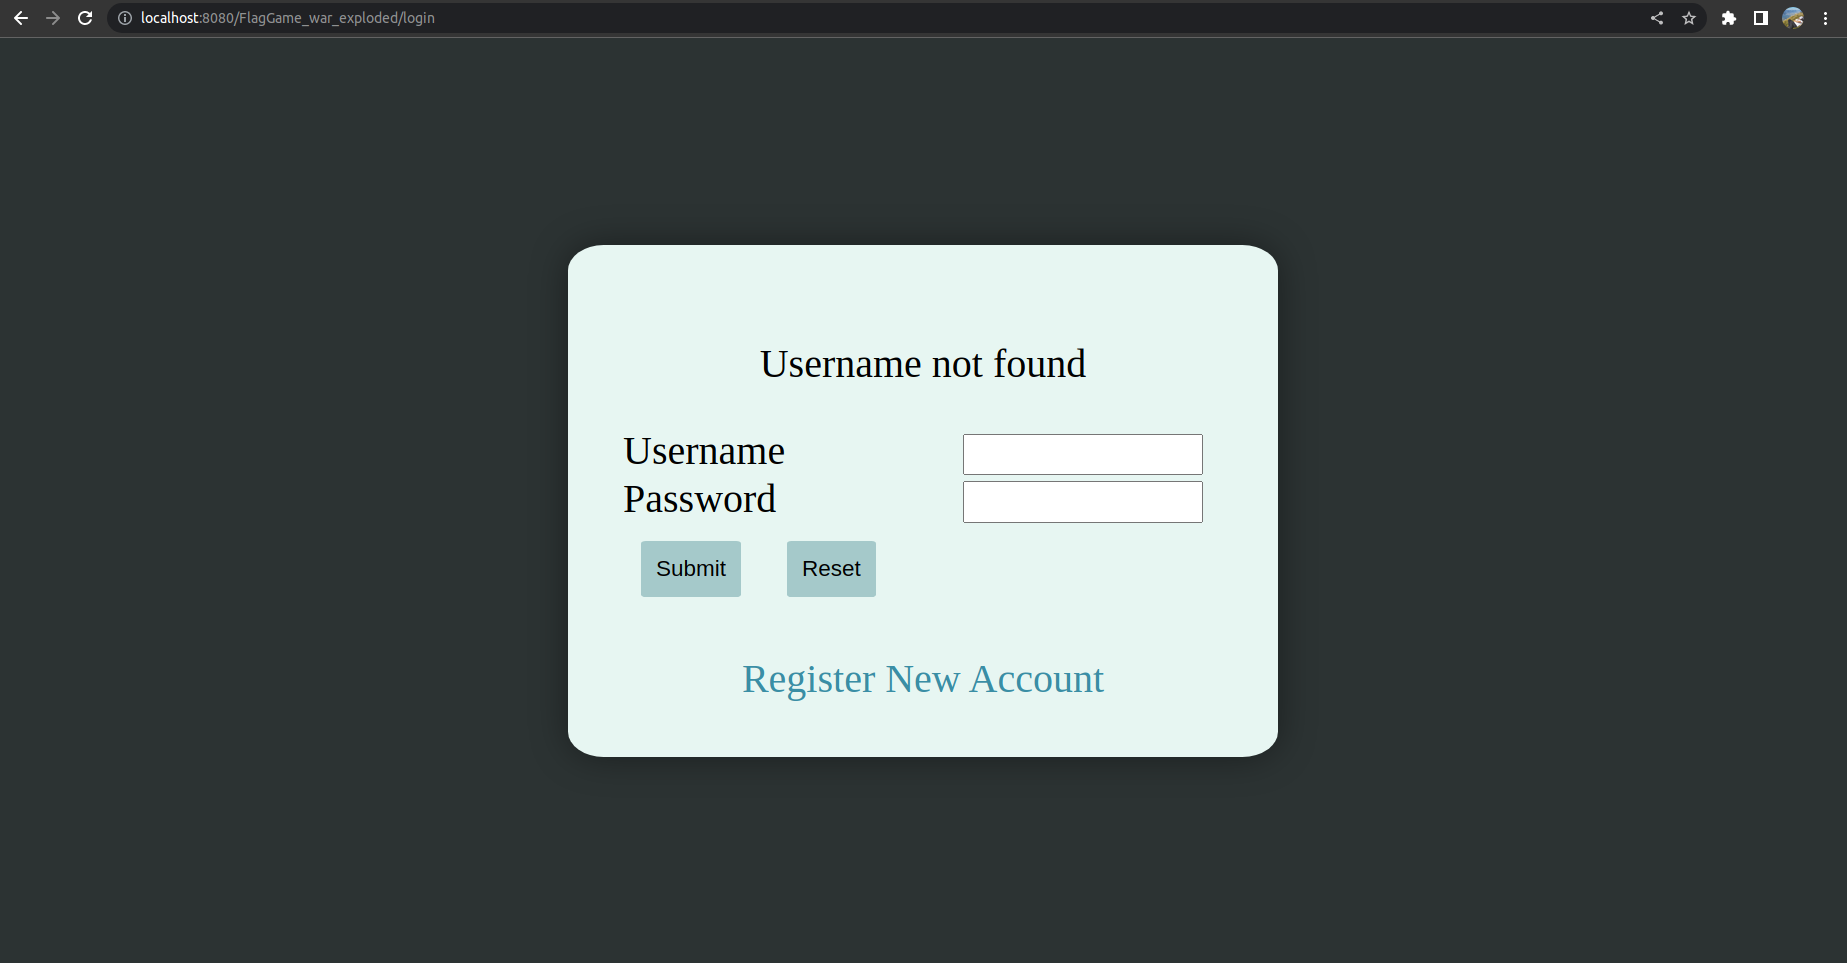
\includegraphics[width=\columnwidth]{login_username_not_found.png}
  \caption{Login Page if the username is not found}
\end{figure}

\subsection{Registration Page}
\subsubsection{register.jsp}
Same logic as \textit{login.jsp}, the only difference is that in the form we have a third field.
\subsubsection{Register.java}
The registration page is very similar: the main difference is that now instead of checking the context for an existing user we add a new one. The checks we do are that the two passwords given are the same and that the username does not already exist.

To get the credentials set and create a new session we use the same functions of \textit{Login.java}, \textit{getUsersFromContext} and \textit{setSession}, so we make these functions static. In particular, at the end of the POST method we modify the context with the new, expanded credentials.


\subsubsection{Screenshots}
\begin{figure}[H]
  \centering
  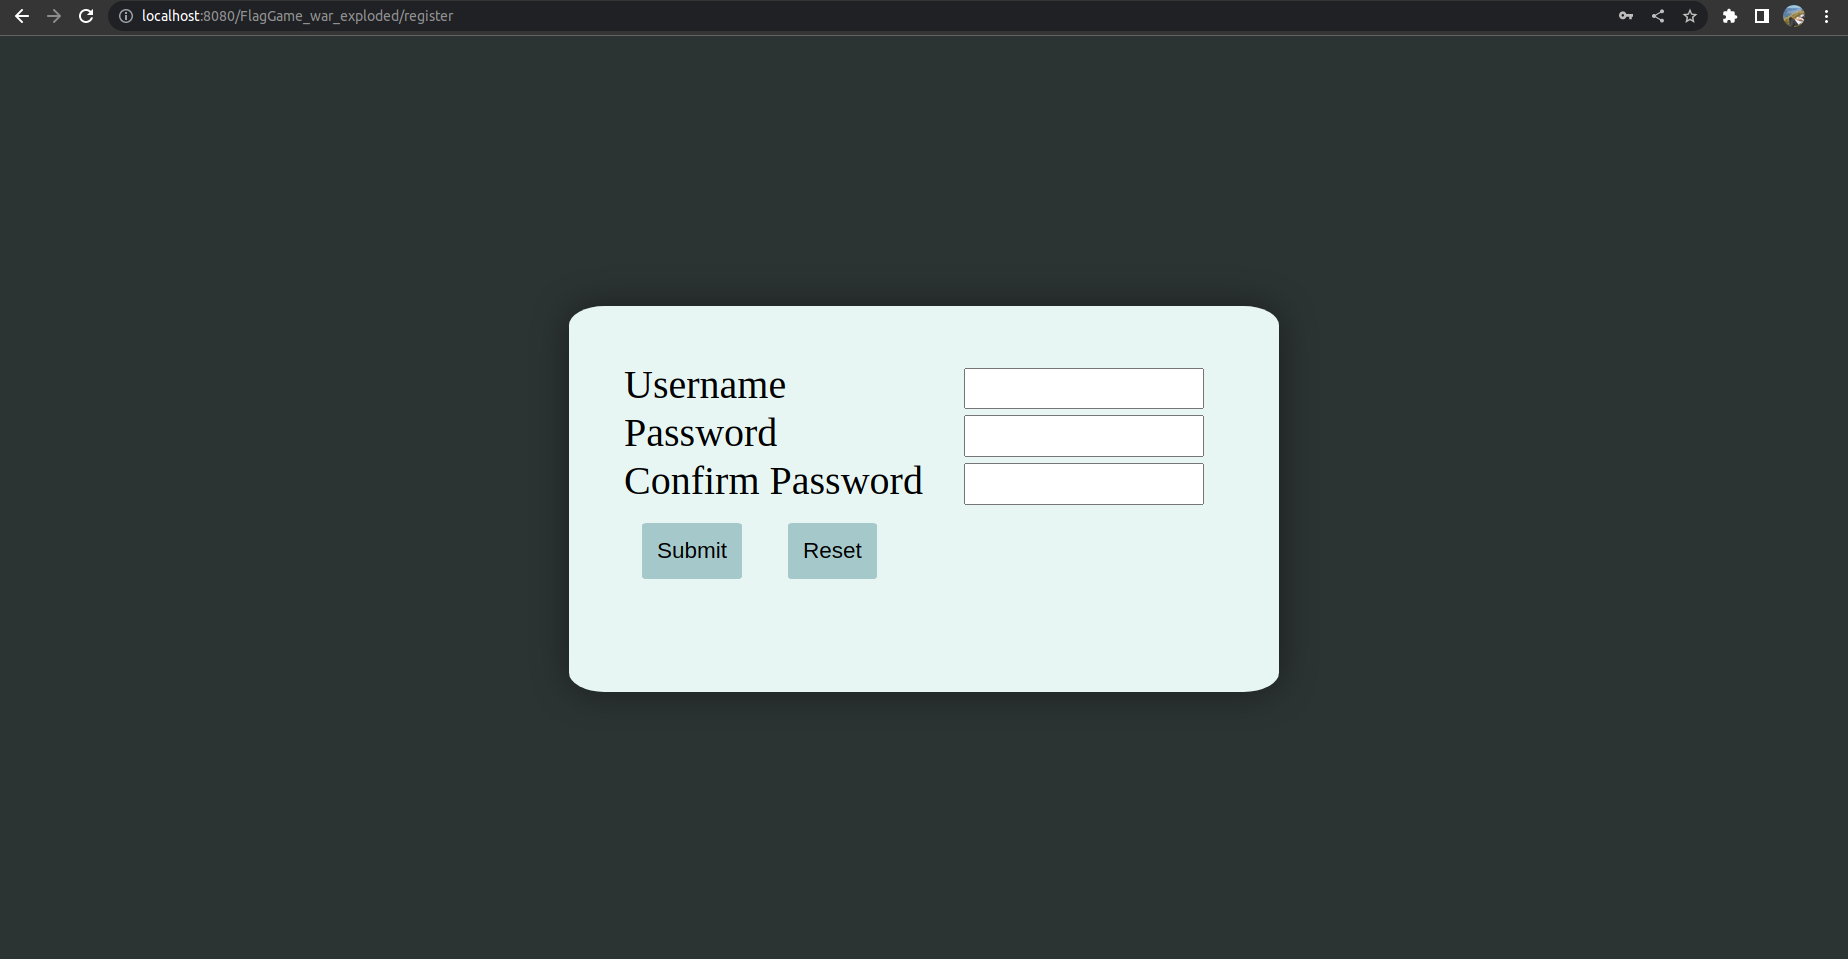
\includegraphics[width=\columnwidth]{register.png}
  \caption{Registration Page}
\end{figure}
\begin{figure}[H]
  \centering
  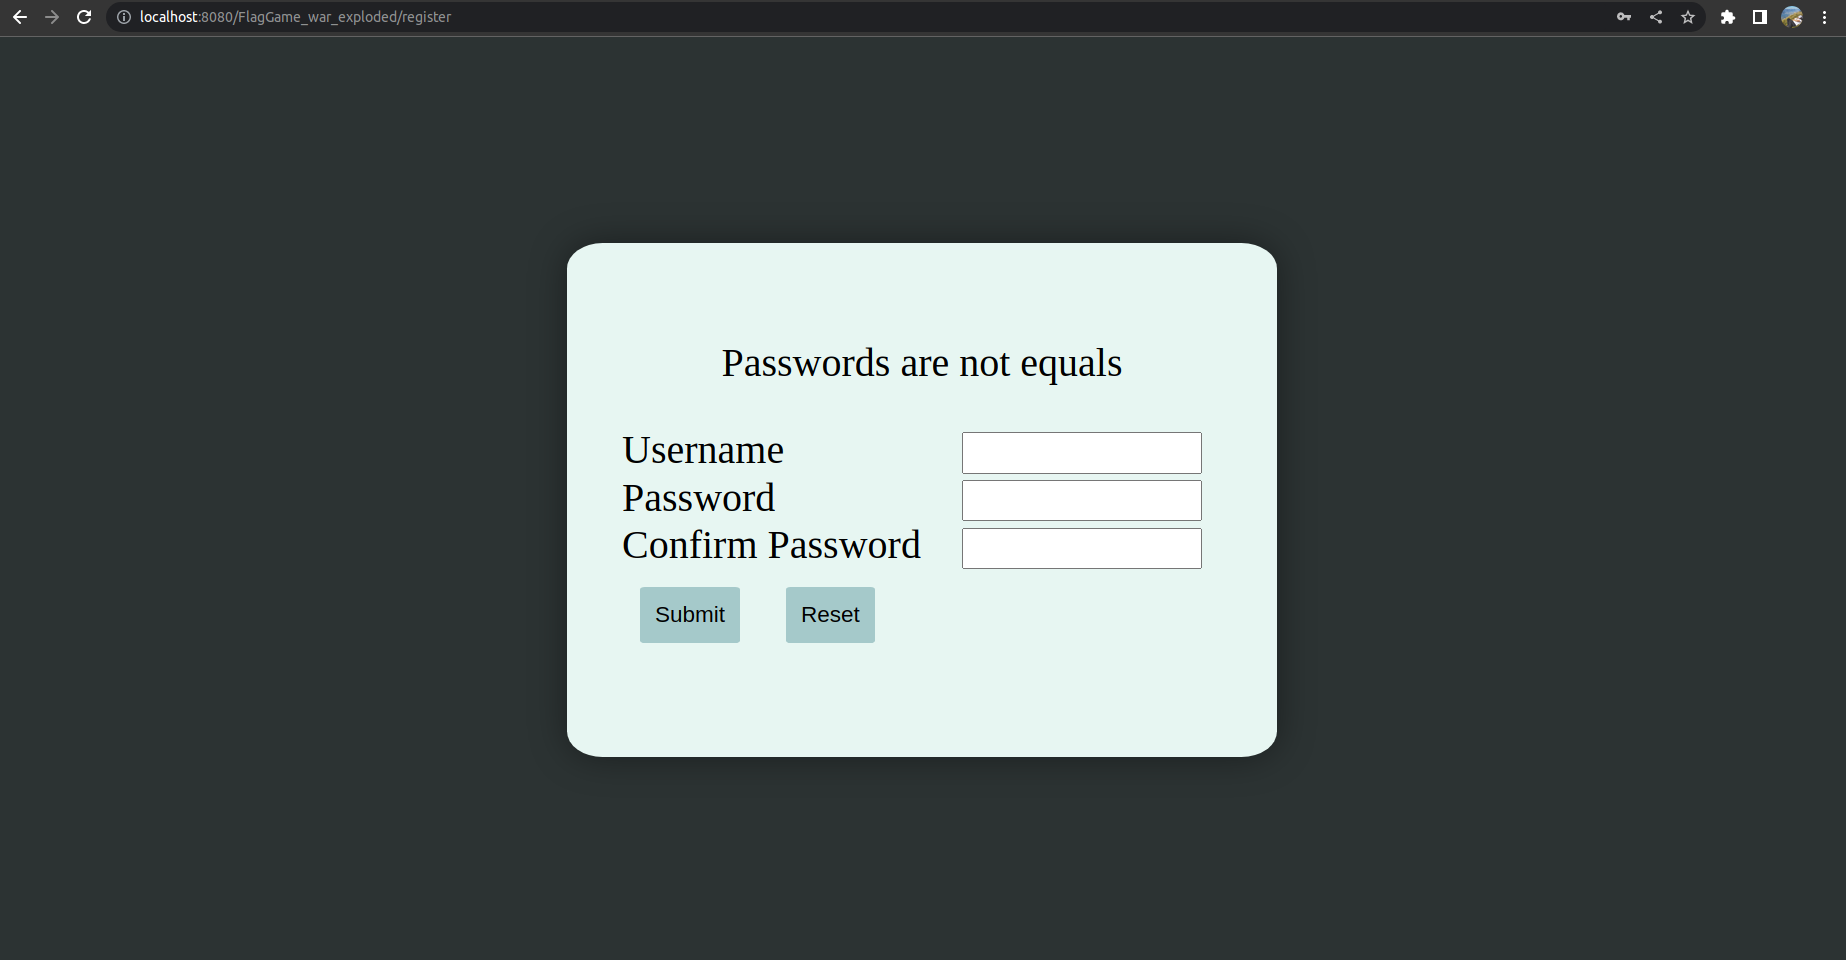
\includegraphics[width=\columnwidth]{register_not_equal_passwords.png}
  \caption{Registration Page if the two passwords given are different}
\end{figure}
\begin{figure}[H]
  \centering
  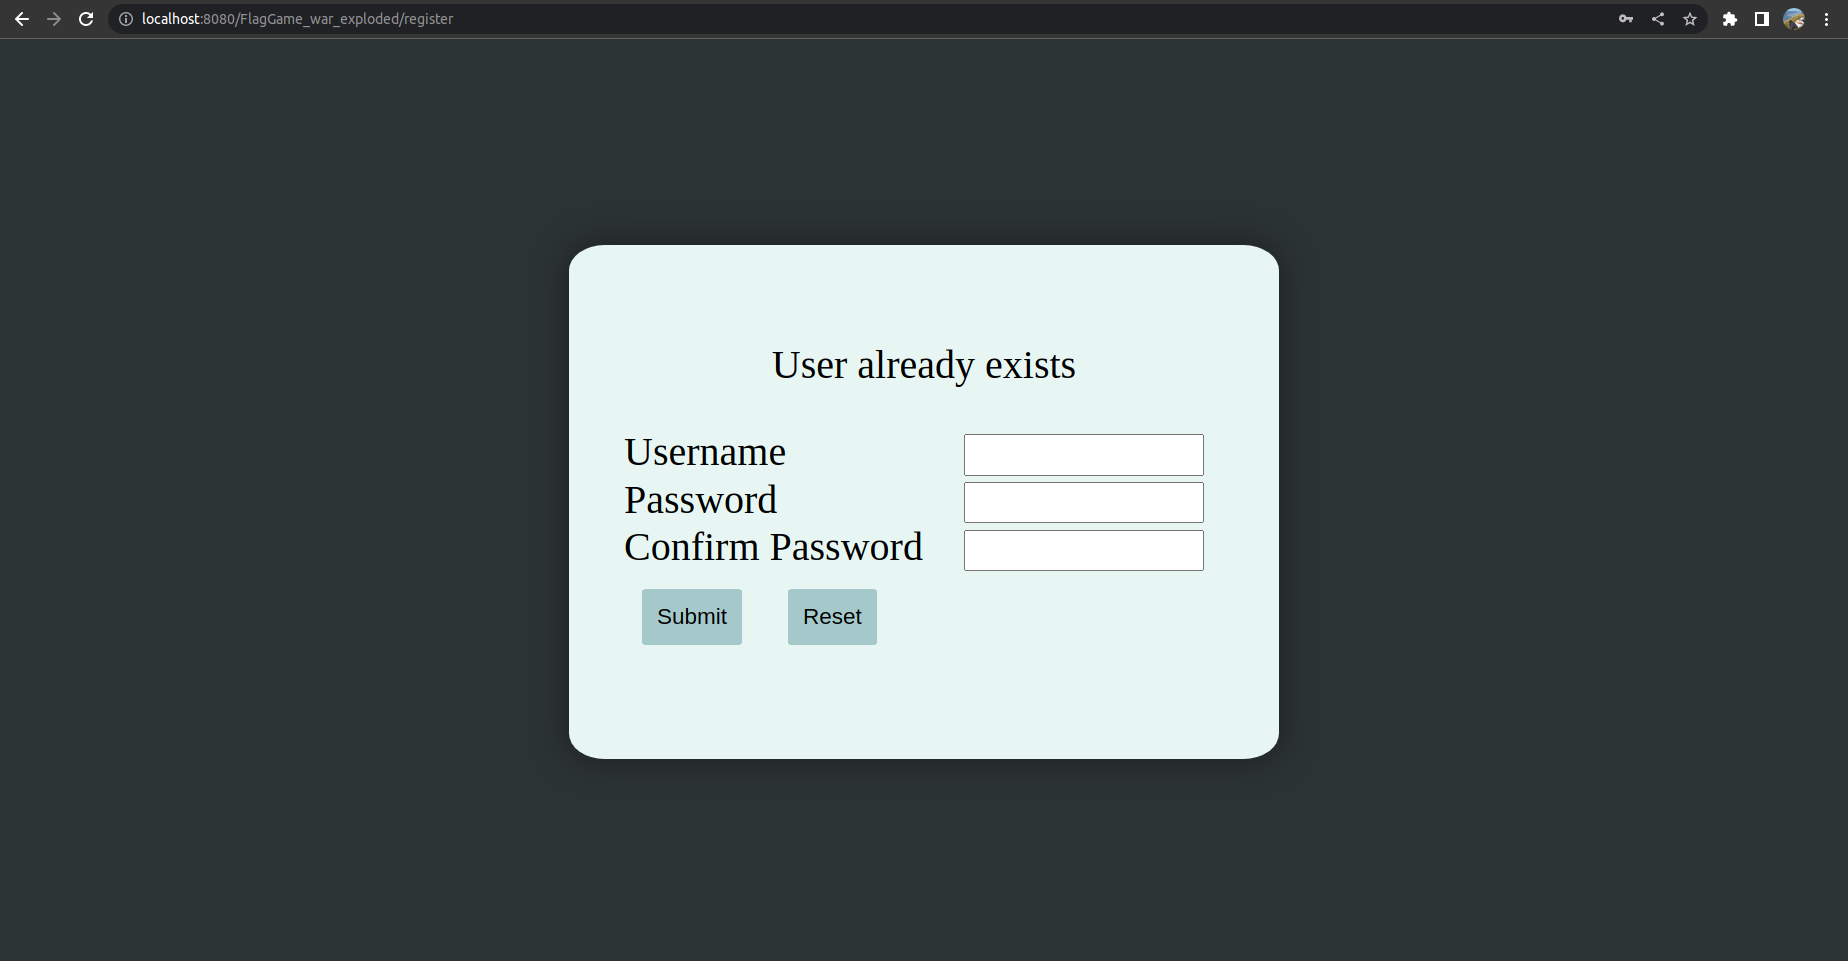
\includegraphics[width=\columnwidth]{register_username_already_exist.png}
  \caption{Registration Page if the username already exists}
\end{figure}
  \section{Task 2, 3 and 7 - Starting page}
\subsection{The task}
We should have a starting page that shows the user name in the header, the points of the user and a button to play the game.

If an unauthenticated user tries to access the page, he gets redirected to the login page.
\subsection{Main page}
\subsubsection{main.jsp}
This page is just an header for the username, a paragraph for the points and a form with a button to redirect to the game page
\subsubsection{Main.java}
This page is set up at the starting url \textit{\/}, so when the user access the webapp he gets automatically redirected to the login page.

The page itself has only one method, GET, which controls the username saved in the session: if not present, redirects to the login page; if it is the admin, redirects to the admin page (as asked in the task 8); otherwise for a normal user forwards the \textit{main.jsp} page.

We also have a static function to get the user session. This function is used by many pages, and what it does is getting the username and the points from the session; if there is no session or the session does not have an username, it redirects to the login page. In this way we can use just this function to implement the task 7.


\subsubsection{Screenshots}
\begin{figure}[H]
  \centering
  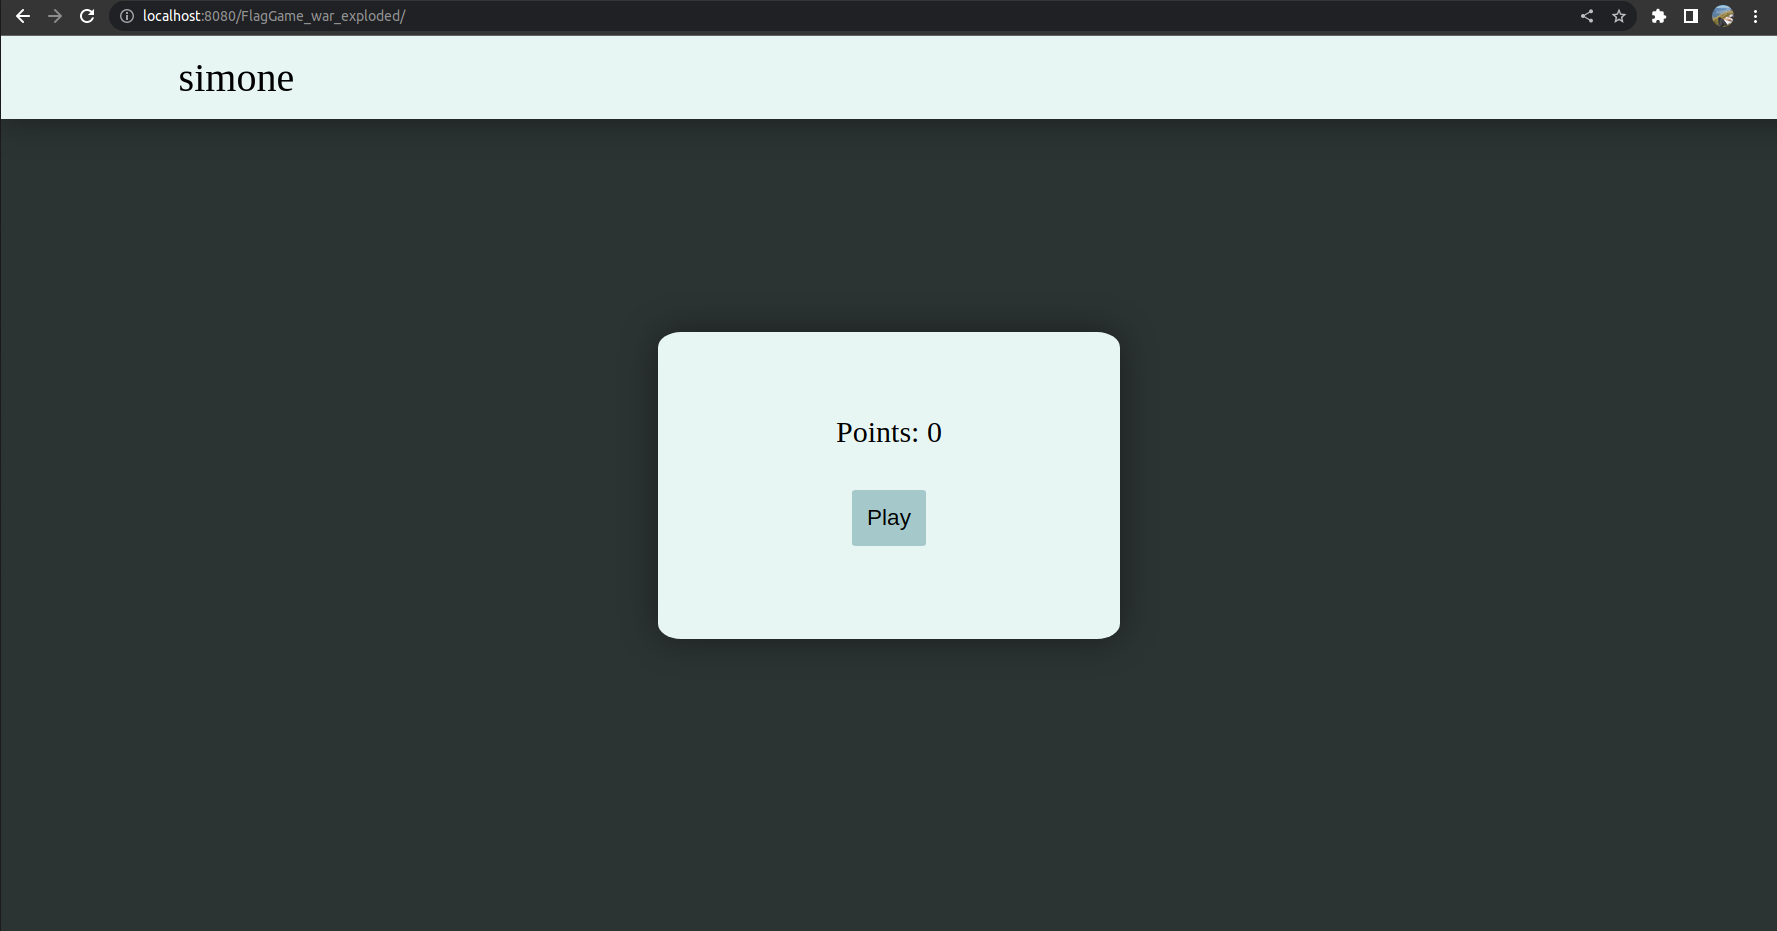
\includegraphics[width=\columnwidth]{main.png}
  \caption{Main Page}
\end{figure}
  \section{Task 4, 5 and 6 - Flag Game}
\subsection{The task}
The game consists of guessing the capitals of three random flags from a given pool.

The user writes the number on the input text near each flag. This number is taken from the shown list of capital cities. All fields must be filled in to submit a guess.

If the answers are correct, it increases the user points by three, otherwise it decreases them by one. It then returns to the main page.
\subsection{Game page}
\subsubsection{game.jsp}
At the start of the page we create a Capitals object: this objects has two fields, \textit{capitals} and \textit{chosen\_capitals}, which are both String arrays. At the object creation, the constructor fills \textit{capitals} with city names and shuffle it, then it chooses three random and add them to \textit{chosen\_capitals}.

We also get the user with the same method from \textit{Main.java}, so that we can be redirected if we do not have an authentication.

In the page, we show the same header as the main page, then an ordered list that shows \textit{capitals} and a form with an entry for each element of \textit{chosen\_capitals}. This form has for each label an image and an input field. The image is saved in the system as \textit{(capital\_name).png}, so it is easy to get it from the chosen capital value. The input field is of type number, required and has value \textit{min=0} and \textit{max=(capitals.lenght())}. The name value is taken from a Capitals method \textit{findCapitalId()}, which takes as an input a city name and returns its index in \textit{capitals}. This way, the url that gets the form results has only to compare the field name and field value.
\subsubsection{Game.java}
The GET method simply redirects to the \textit{game.jsp} page.

The POST method, as sad before, compares the field names and values to determine if the user got all responses correctly. It then updated the user session and the context (as asked for task 8) and redirects to the main page.


\subsubsection{Screenshots}
\begin{figure}[H]
  \centering
  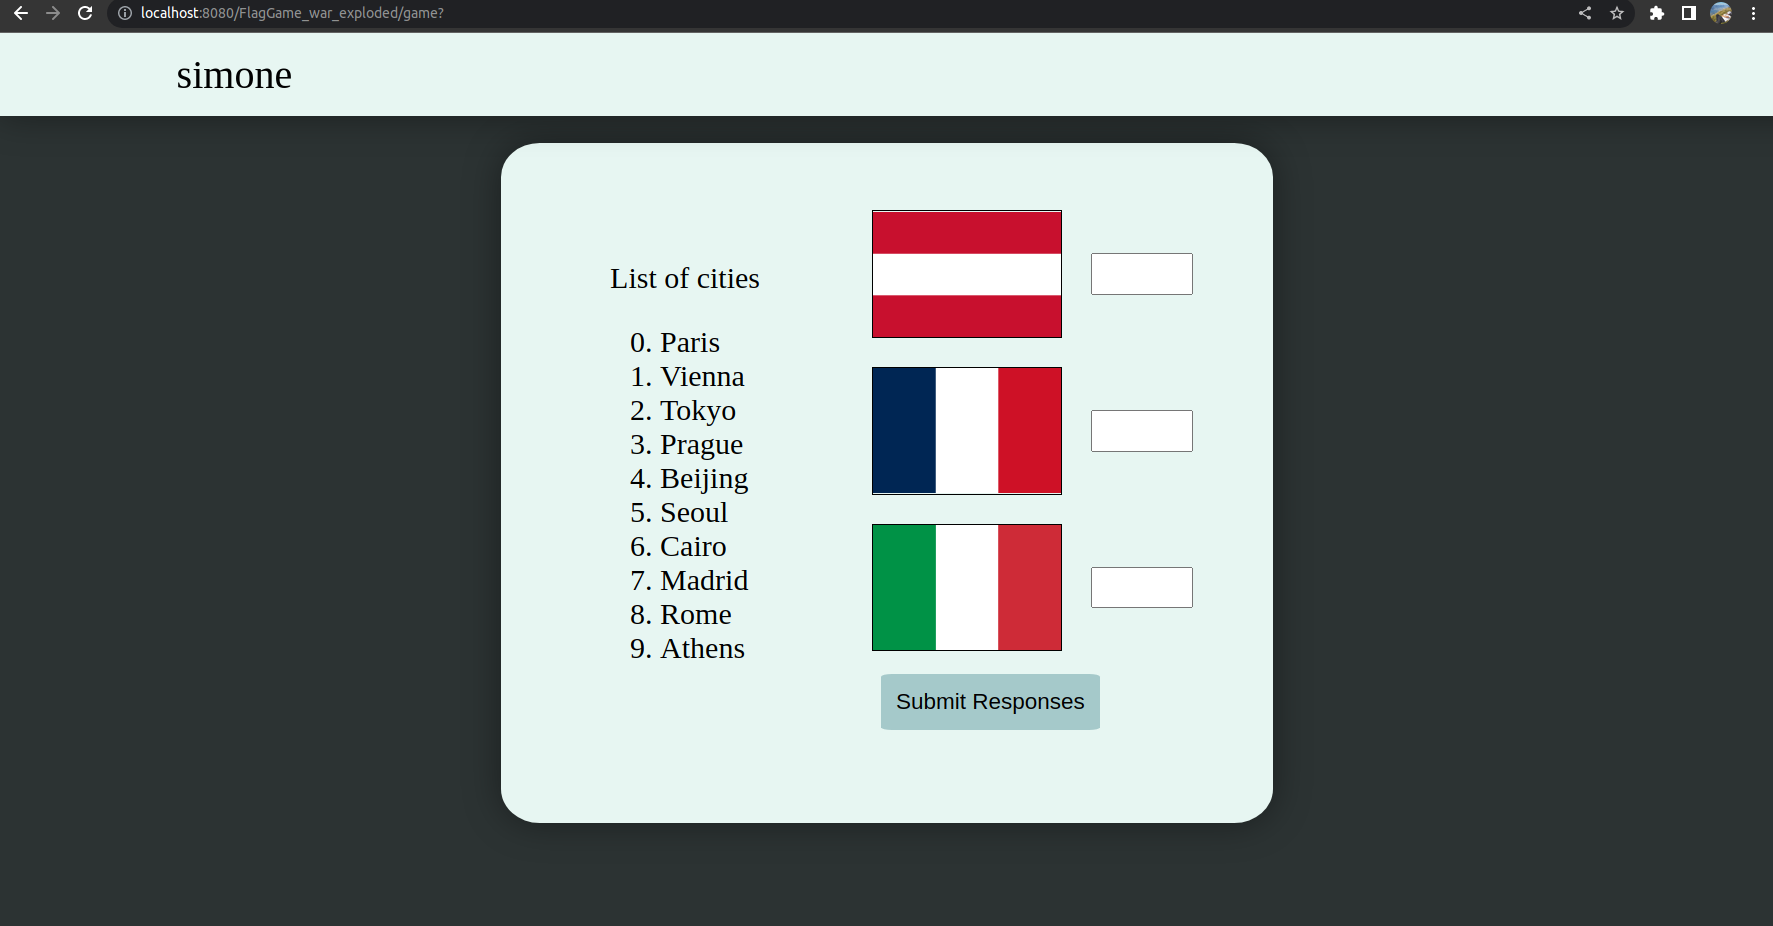
\includegraphics[width=\columnwidth]{game_1.png}
  \caption{Flag Game}
\end{figure}
\begin{figure}[H]
  \centering
  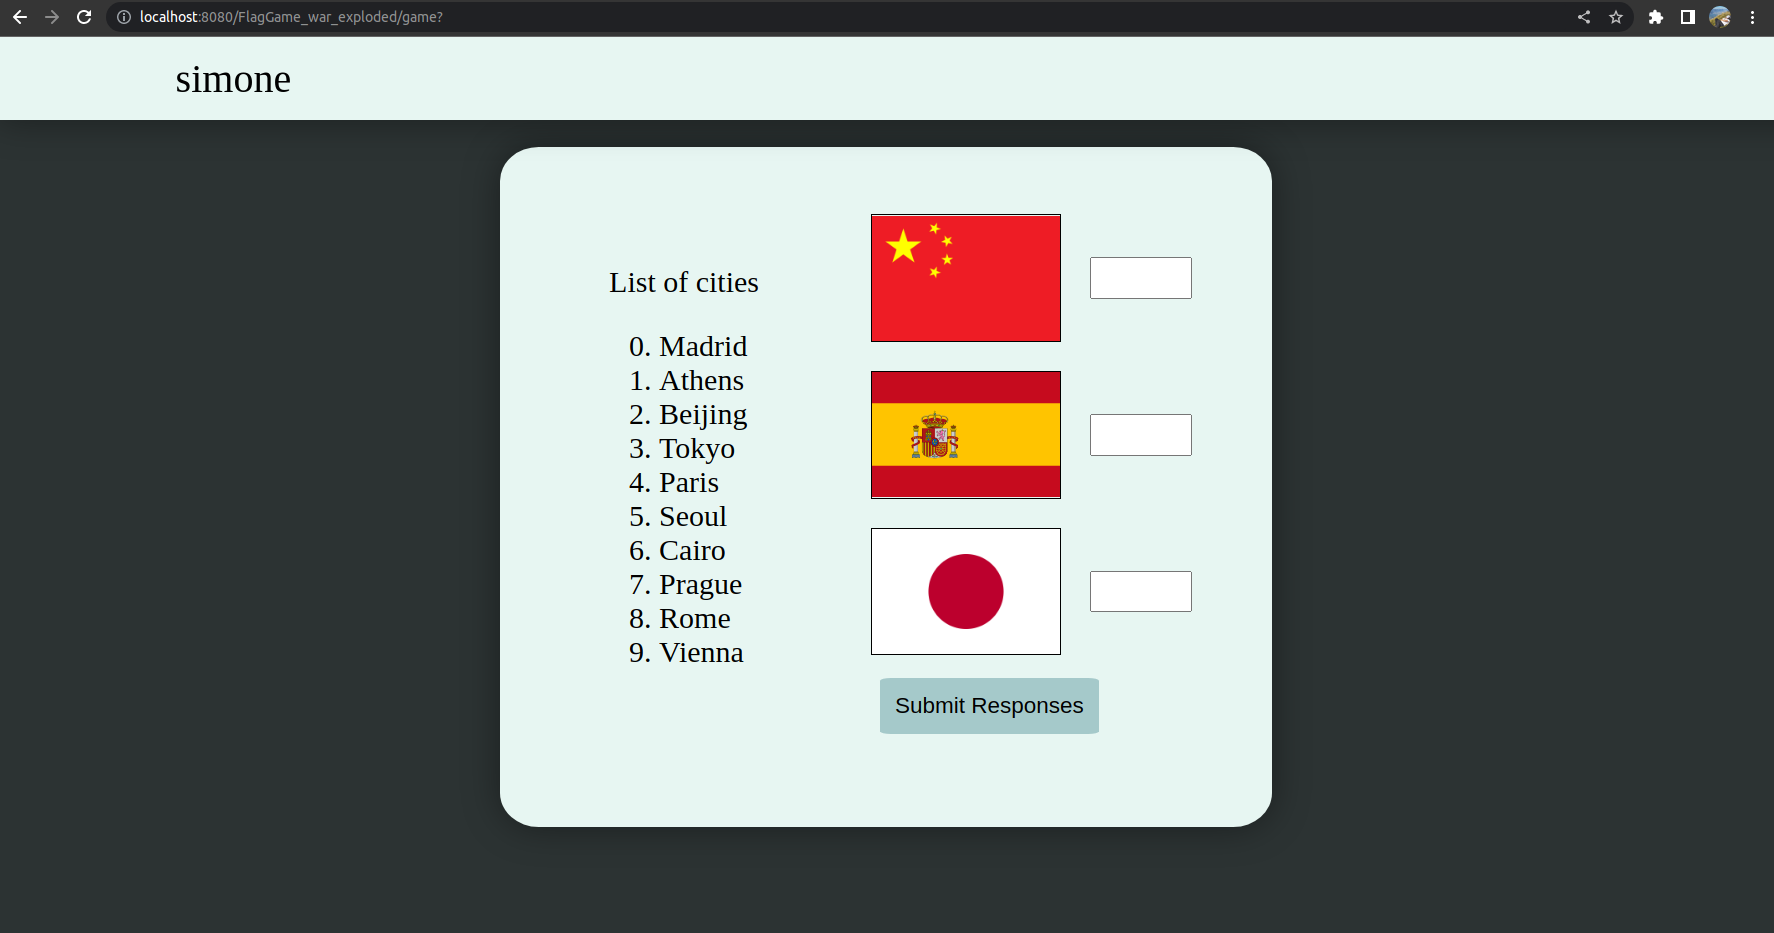
\includegraphics[width=\columnwidth]{game_2.png}
  \caption{Flag Game, another example}
\end{figure}
  \section{Task 8 - Admin}
\subsection{The task}
The admin (with defined credentials admin, password nimda) should be redirected from the main page to an admin page where he can see the current logged users and their points.

If a normal user tries to access the page, it returns error code 401. (Note: the correct code to return should be 403 Forbidden and not 401 Unauthorized, but we will follow the assignment request).
\subsection{Sessions in the Context}
Since we do not have a native method to get all the current sessions of our system, we need to save them in the servlet context each time a session is created (login or registration) or updated (points given at the end of a game).

Since the context is shared memory, all the functions that modify it should be in a synchronized block.
\subsubsection{Create or update Session}
A new session creation is done by the function \textit{Login.setSession()}. Here, we get the context, add the new session and update it. If the session already has an username, it means that the user is doing another login, so we update the session username value. At the same time, we search the context for the old session and delete it, before adding a new one. In this way, we do not have multiple open sessions in the context for an user that changes credentials. (Note: for this reason, during testing accessing first as an user and then as an admin deletes the first session and the admin page would only show the admin as online. It is needed to log in as the user from another browser or from a private/incognito page, which uses different sessions).

A session update is also done by the game page to update the points. In this case, we search in the context for the user session and update the points there too.
\subsubsection{SessionListener.java}
If a session ends, we need to remove it from the context. This can be done with an \textit{HttpSessionListener}. We can implement it with the class \textit{SessionListener.java}, where we simply search for the expired session username and delete it from the context.


\subsection{Admin page}
\subsubsection{admin.jsp}
The admin jsp page takes as an argument the list of users to show. It contains a simple table with three columns: rank, username and points. The reason for the rank column is that we set up the list of users to be ordered, but this was not required.

This page does not redirect if a simple user tries to access the file directly instead of passing first by the java class. It is not a problem, however, since the page itself does not have the capability to access the context and gather the sensitive data.
\subsubsection{unauthorized.jsp}
This page simply shows an error message and a link to return to the main page.
\subsubsection{Admin.java}
If the user is not authenticated, redirects to the main page with the static method \textit{Main.getUserSession}. 

If the username is not the admin one (set up by a static variable \textit{ADMIN\_USERNAME} because needed also by \textit{Main.java}), it redirects to \textit{unauthorized.jsp}. 

If the user is the admin, it gets all the session saved in the context, sort them and forward them to \textit{admin.jsp}


\subsubsection{Screenshots}
\begin{figure}[H]
  \centering
  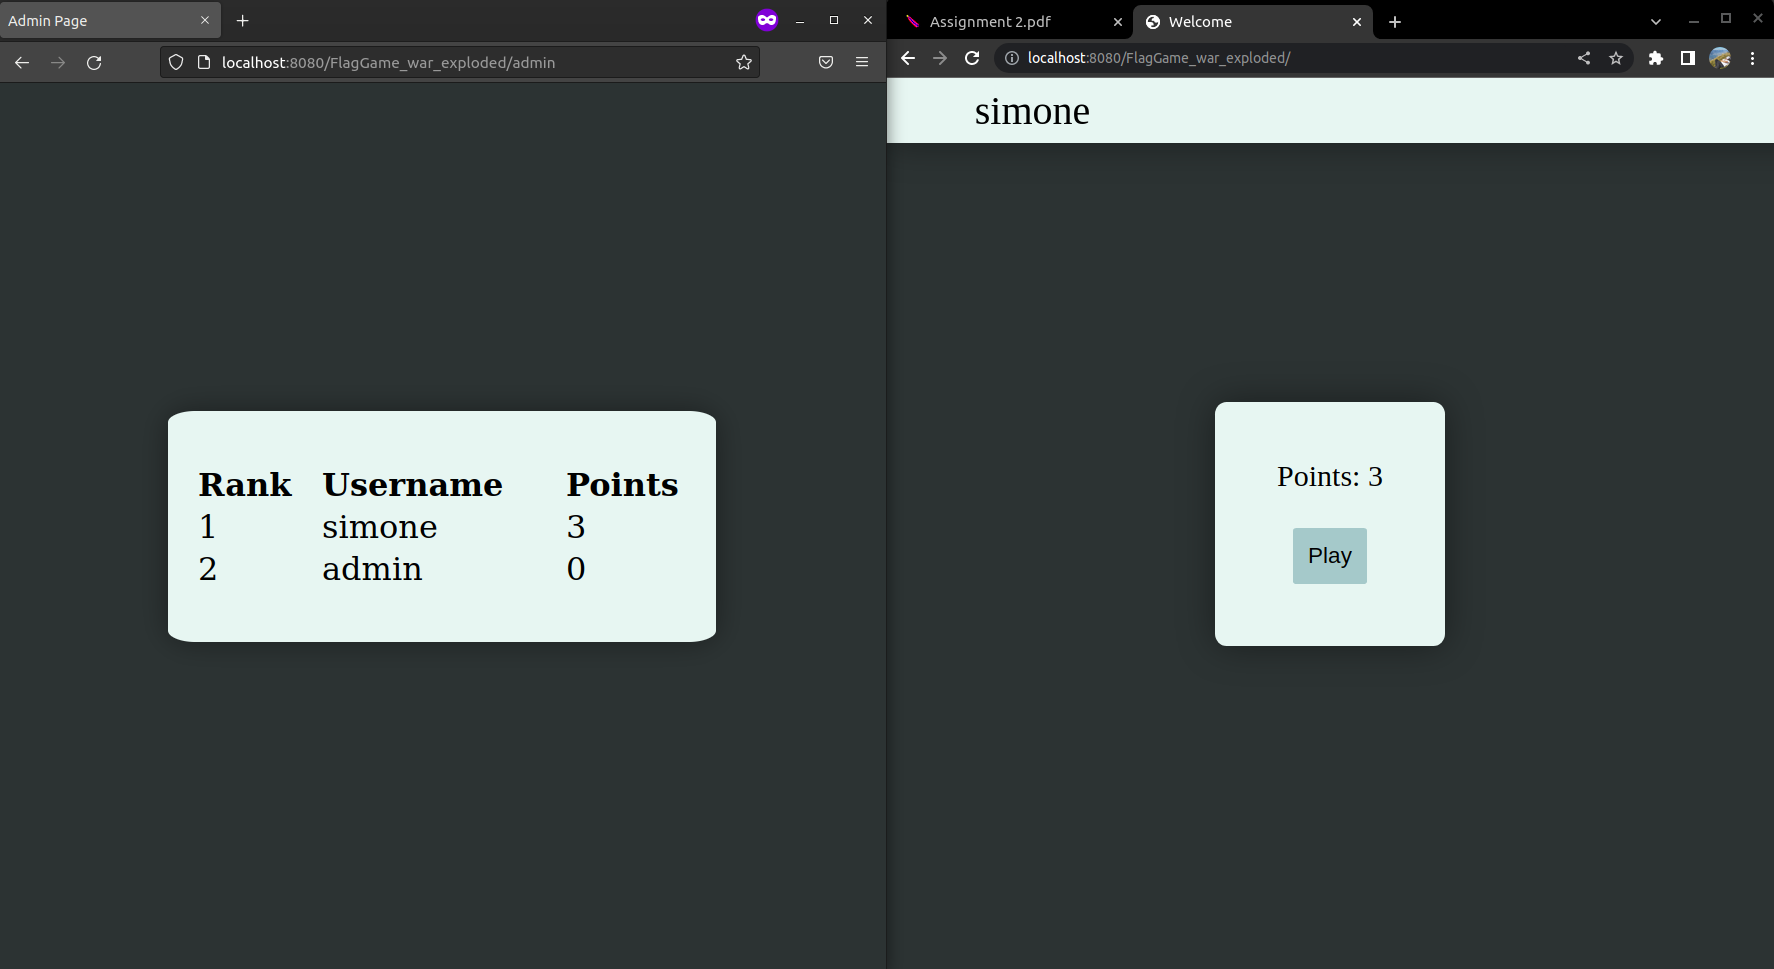
\includegraphics[width=\columnwidth]{admin.png}
  \caption{Admin page and an user main page}
\end{figure}
\begin{figure}[H]
  \centering
  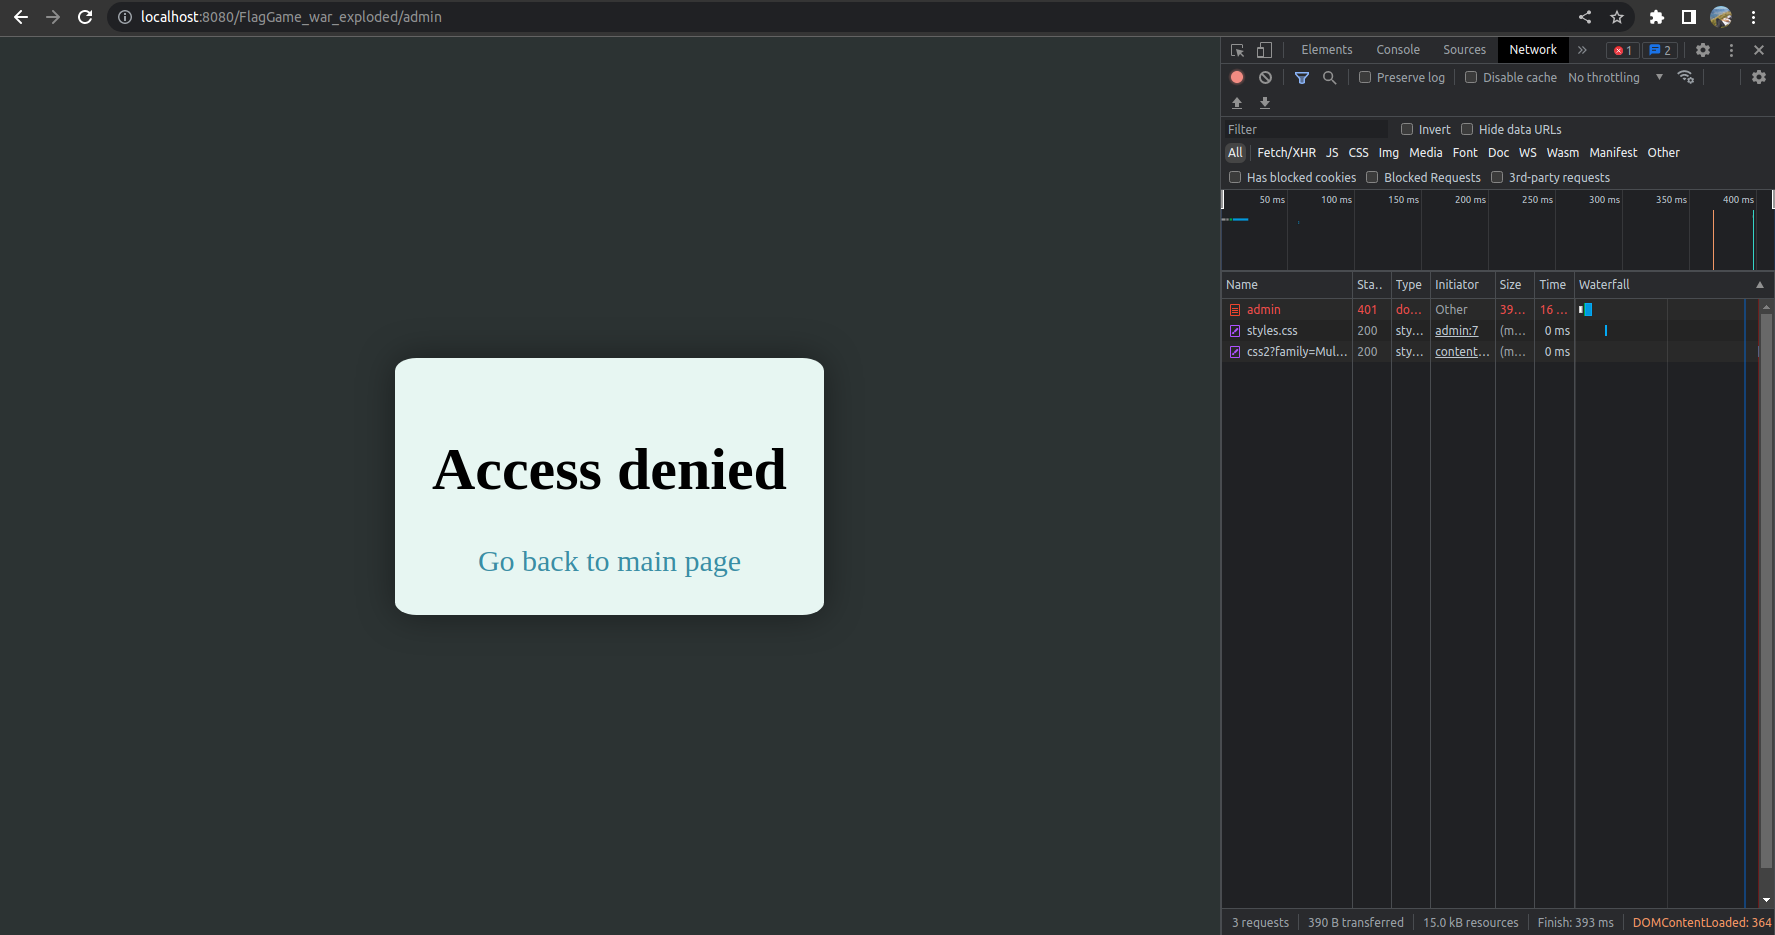
\includegraphics[width=\columnwidth]{unauthorized.png}
  \caption{Unauthorized page. The status code is 401}
\end{figure}
  \section{Task 9 - Persistent Credentials}
\subsection{The task}
The credentials are mantained as long as the webapp is running. When shutdown, they should be saved to a file and recovered at the next redeploy.
\subsection{Servlet Context Listener}
We can execute actions when the servlet is turned on or off with the servlet context listener, which uses two methods: \textit{contextInitialized} and \textit{contextDestroyed}.
\subsubsection{ContextListener.java}
When the servlet is turned on, we read the data from the file. If the file does not exist or the file cannot be opened, we create a new context with the admin and another starting user; otherwise we add to the context the users we read.

When the servlet is turned off, we save all the user credentials saved in the context inside the file.


\subsubsection{Screenshots}
\begin{figure}[H]
  \centering
  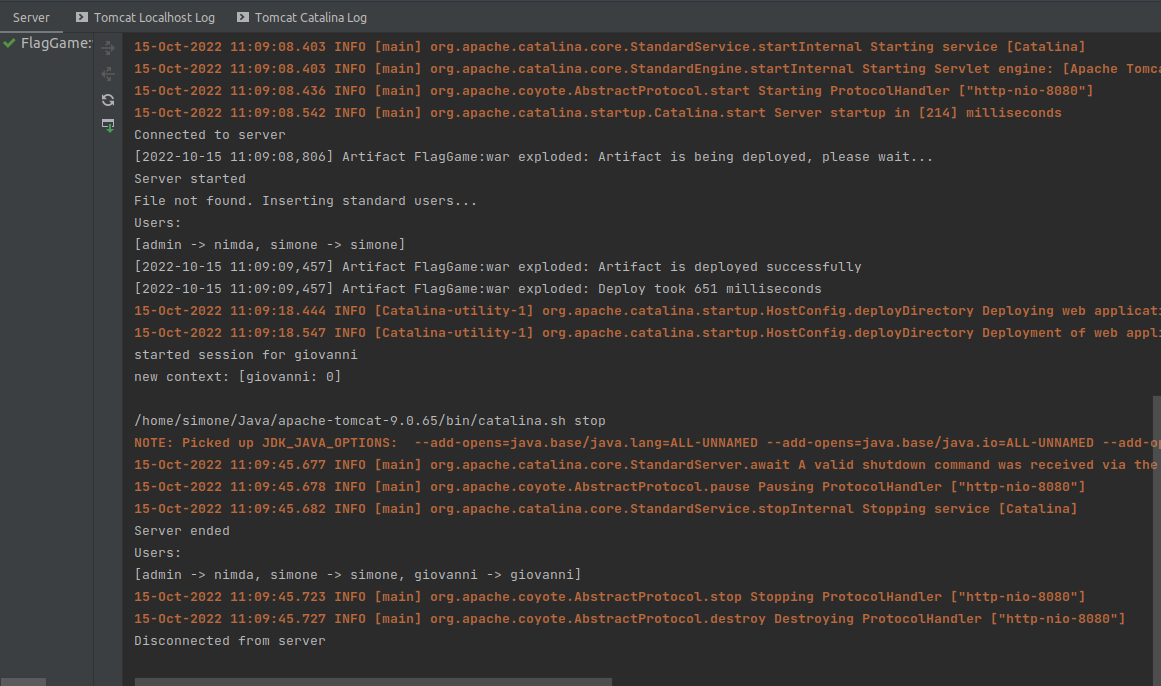
\includegraphics[width=\columnwidth]{context_new.png}
  \caption{When the file is not found, a standard context is created. We then create a new User, and we can see how it also get saved at the server shutdown}
\end{figure}
\begin{figure}[H]
  \centering
  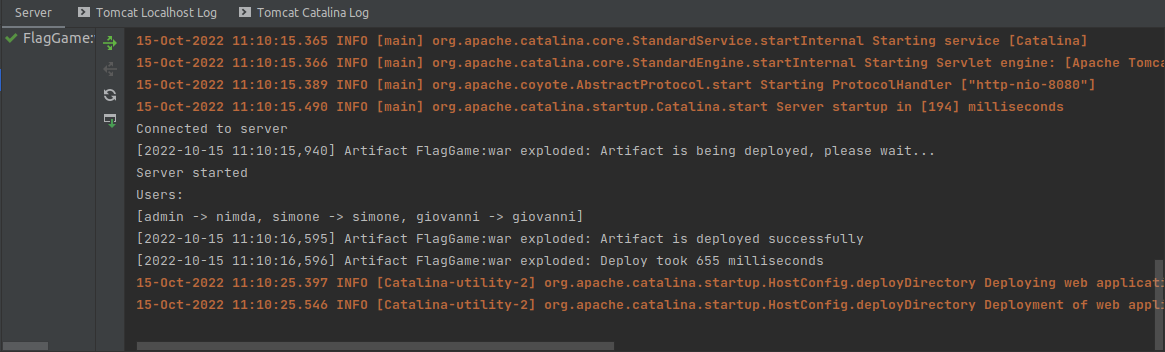
\includegraphics[width=\columnwidth]{context_read.png}
  \caption{At the next redeploy, the three users get correctly recovered}
\end{figure}

  \pagebreak
  \section{Code snippets}
Below some snippets of code to better understand the project
\subsection{Login.java code}
\begin{lstlisting}[language=java, caption={method to get the user credentials from the context}]
public static synchronized List<UserCredentials> getUsersFromContext(ServletContext context) {
    Object usersAttribute =  context.getAttribute("users");
    @SuppressWarnings("unchecked")
    List<UserCredentials> userCredentials = (List<UserCredentials>) usersAttribute;
    return userCredentials;
}
\end{lstlisting}
\begin{lstlisting}[language=java, caption={method to set the user session}]
public static synchronized void setSession(HttpServletRequest req, String username, ServletContext context){
    System.out.println("started session for " + username);

    Object loggedAttribute =  context.getAttribute("logged");
    @SuppressWarnings("unchecked")
    List<UserSession> logged = (ArrayList<UserSession>) loggedAttribute;
    if (logged == null) logged = new ArrayList<>();

    HttpSession session = req.getSession();

    // if the user already had a session
    String old_username = (String) session.getAttribute("username");
    if (old_username != null) {
        System.out.println("old login to delete: " + old_username);
        UserSession old_session = new UserSession(old_username, 0);
        logged.remove(old_session);
    }

    session.setAttribute("username", username);
    session.setAttribute("points", 0);
    UserSession new_session = new UserSession(username, 0);

    logged.add(new_session);
    System.out.println("new context: " + logged);
    System.out.println();
    context.setAttribute("logged", logged);
} 
\end{lstlisting}
\begin{lstlisting}[language=java, caption={POST method for login page}]
protected void sendLoginForm(HttpServletRequest req, HttpServletResponse res, String error_msg) throws IOException, ServletException {
      req.setAttribute("error_msg", error_msg);
      req.getRequestDispatcher("jsp/login.jsp").forward(req, res);
}

@Override
protected void doPost(HttpServletRequest req, HttpServletResponse res) throws IOException, ServletException {
    String username = req.getParameter("username");
    String password = req.getParameter("password");

    List<UserCredentials> userCredentials;
    synchronized (getServletContext()) {
        ServletContext context = getServletContext();
        userCredentials = getUsersFromContext(context);
    }
    Iterator<UserCredentials> iter = userCredentials.iterator();
    boolean found = false;
    while (iter.hasNext()) {
        UserCredentials user = iter.next();
        if (user.getUsername().equals(username)) {
          found = true;
          if (!user.getPassword().equals(password)) {
              // password not correct
              sendLoginForm(req, res, "Password not correct");
              return;
          }
          // account verified
          break;
        }
    }
    if (!found) {
        // username not found
        sendLoginForm(req, res, "Username not found");
        return;
    }

    synchronized (getServletContext()) {
        ServletContext context = getServletContext();
        setSession(req, username, context);
    }

    res.sendRedirect(req.getContextPath());
}
\end{lstlisting}
\subsection{Register.java code}
\begin{lstlisting}[language=java, caption={POST method for registration page}]
protected void sendRegisterForm(HttpServletRequest req, HttpServletResponse res, String error_msg) throws IOException, ServletException {
    req.setAttribute("error_msg", error_msg);
    req.getRequestDispatcher("jsp/register.jsp").forward(req, res);
}

@Override
protected void doPost(HttpServletRequest req, HttpServletResponse res) throws IOException, ServletException {
    String username = req.getParameter("username");
    String password = req.getParameter("password");
    String confirm_password = req.getParameter("confirm_password");

    if(!password.equals(confirm_password)) {
        sendRegisterForm(req, res, "Passwords are not equals");
        return;
    }

    List<UserCredentials> userCredentials;
    synchronized (getServletContext()) {
        ServletContext context = getServletContext();
        userCredentials = Login.getUsersFromContext(context);
    }

    // check the user does not already exist
    for (UserCredentials user : userCredentials) {
        if (user.getUsername().equals(username)) {
            sendRegisterForm(req, res, "User already exists");
            return;
        }
    }

    userCredentials.add(new UserCredentials(username, password));
    synchronized (getServletContext()) {
        ServletContext context = getServletContext();
        context.setAttribute("users", userCredentials);
        Login.setSession(req, username, context);
    }

    res.sendRedirect(req.getContextPath());
}
\end{lstlisting}
\subsection{Main.java code}
\begin{lstlisting}[language=java, caption={method to get the user from the session}]
public static synchronized UserSession getUserSession(HttpServletRequest req, HttpServletResponse res) throws IOException {
    HttpSession session = req.getSession();
    String username = (String) session.getAttribute("username");
    if(username == null) {
        res.sendRedirect("login");
        return null;
    }
    int points = (int) session.getAttribute("points");
    return new UserSession(username, points);
}
\end{lstlisting}
\begin{lstlisting}[language=java, caption={GET method for main page}]
@Override
public void doGet(HttpServletRequest req, HttpServletResponse res) throws IOException, ServletException {
    UserSession user = getUserSession(req, res);
    if (user == null) return;
    if (user.getUsername().equals(Admin.ADMIN_USERNAME)) {
        res.sendRedirect("admin");
        return;
    }

    req.getRequestDispatcher("jsp/main.jsp").forward(req, res);
}
\end{lstlisting}
\subsection{Game code}
\begin{lstlisting}[language=java, caption={POST method for game page}]
@Override
protected void doPost(HttpServletRequest req, HttpServletResponse res) throws IOException {
    UserSession user = Main.getUserSession(req, res);
    if (user == null) return;

    Enumeration<String> param_names = req.getParameterNames();
    boolean guessed_all = true;
    while(param_names.hasMoreElements()){
        String param_name = param_names.nextElement();
        String param_value = req.getParameter(param_name);
        if(!param_value.equals(param_name)){
            guessed_all = false;
            break;
        }
    }

    int added_points = 0;
    if(guessed_all) added_points = 3;
    else if(user.getPoints() > 0) added_points = -1;
    user.setPoints(user.getPoints() + added_points);

    synchronized (getServletContext()) {
        ServletContext context = getServletContext();
        Object loggedAttribute =  context.getAttribute("logged");
        @SuppressWarnings("unchecked")
        List<UserSession> logged = (ArrayList<UserSession>) loggedAttribute;

        for (UserSession logged_user: logged) {
            if(logged_user.getUsername().equals(user.getUsername())) {
                logged_user.setPoints(user.getPoints());
                break;
            }
        }

        System.out.println(user.getUsername() + " made " + added_points + " points");
        System.out.println("new context: " + logged);
        System.out.println();
        context.setAttribute("logged", logged);
    }

    HttpSession session = req.getSession();
    session.setAttribute("points", user.getPoints());
    res.sendRedirect(req.getContextPath());
}
\end{lstlisting}
\begin{lstlisting}[language=html, caption={game.jsp code}]
<%
  Capitals cap = new Capitals();
  UserSession userCredentials = Main.getUserSession(request, response);
  if (userCredentials == null) return;
%>
<html>
<head>
  <title>Flag Game</title>
  <link rel="stylesheet" href="styles.css"/>
</head>
<body class="game-body">
  <header><%=userCredentials.getUsername()%></header>

  <div class="capitals-list">
      <p>List of cities</p>
      <ol start="0">
          <% for(String capital: cap.getCapitals()) { %>
          <li><%=capital%></li>
          <% } %>
      </ol>
  </div>

  <form action="game" method="POST" class="game-form">
      <% for(String capital: cap.getChosenCapitals()){ %>
          <div class="game-input">
              <label for="<%=capital%>">
                  <img 
                      src="flags/<%=capital%>.png" 
                      width="150" 
                      height="100" 
                      alt="Refresh the page"
                  />
              </label>
              <input 
                  id="<%=capital%>"
                  name="<%=cap.findCapitalId(capital)%>"
                  type="number" 
                  required min="0" 
                  max="<%=cap.getNCapitals()%>"
              />
          </div>
      <% } %>
      <button type="submit">Submit Responses</button>
  </form>
</body>
</html>
\end{lstlisting}
\subsection{SessionListener.java code}
\begin{lstlisting}[language=java, caption={listener of session changes}]
@WebListener
public class SessionListener implements HttpSessionListener {
    @Override
    public void sessionDestroyed(HttpSessionEvent se) {
        HttpSession old_session = se.getSession();
        String username = (String) old_session.getAttribute("username");
        System.out.println("Finished session for " + username);
        UserSession old_user_session = new UserSession(username, 0);

        synchronized (old_session.getServletContext()) {
            ServletContext context = old_session.getServletContext();
            Object loggedAttribute =  context.getAttribute("logged");
            @SuppressWarnings("unchecked")
            List<UserSession> logged = (ArrayList<UserSession>) loggedAttribute;
            logged.remove(old_user_session);
            System.out.println("new context: " + logged);
            System.out.println();
            context.setAttribute("logged", logged);
        }
    }
}
\end{lstlisting}
\subsection{Admin.java code}
\begin{lstlisting}[language=java, caption={method to get the logged users in the context}]
public List<UserSession> getLoggedUser() {
    synchronized (getServletContext()) {
        ServletContext context = getServletContext();
        Object loggedAttribute = context.getAttribute("logged");
        @SuppressWarnings("unchecked")
        List<UserSession> logged = (ArrayList<UserSession>) loggedAttribute;
        Collections.sort(logged);
        return logged;
    }
}
\end{lstlisting}
\begin{lstlisting}[language=java, caption={GET method for admin page}]
@Override
protected void doGet(HttpServletRequest req, HttpServletResponse res) throws IOException, ServletException {
    UserSession user = Main.getUserSession(req, res);
    if (user == null) return;
    if (!user.getUsername().equals(ADMIN_USERNAME)) {
        res.setStatus(401);
        req.getRequestDispatcher("jsp/unauthorized.jsp").forward(req, res);
        return;
    }

    List<UserSession> logged = getLoggedUser();
    req.setAttribute("logged", logged);
    req.getRequestDispatcher("jsp/admin.jsp").forward(req, res);
}
\end{lstlisting}
\subsection{ContextListener.java code}
\begin{lstlisting}[language=java, caption={listener of context changes}]
@WebListener
public class ContextListener implements ServletContextListener {
    String FILENAME = "Users.txt";

    /** if there is an error reading FILENAME, initialize the servlet as new with standard users */
    public void startNewServer(List<UserCredentials> userCredentials, String error_msg) {
        System.out.println(error_msg + ". Inserting standard users...");
        userCredentials.add(new UserCredentials(Admin.ADMIN_USERNAME, "nimda"));
        userCredentials.add(new UserCredentials("simone", "simone"));
    }
    
    @Override
    public void contextInitialized(ServletContextEvent contextEvent) {
        System.out.println("Server started");
        List<UserCredentials> userCredentials = new ArrayList<>();

        try {
            FileInputStream f = new FileInputStream(FILENAME);
            ObjectInputStream o = new ObjectInputStream(f);

            // Read objects
            while (f.available() > 0) {
                UserCredentials user = (UserCredentials) o.readObject();
                userCredentials.add(user);
            }

            o.close();
            f.close();
        } catch (FileNotFoundException e) {
            startNewServer(userCredentials, "File not found");
        } catch (IOException e) {
            startNewServer(userCredentials, "Error initializing stream");
        } catch (ClassNotFoundException e) {
            startNewServer(userCredentials, "File has not correct format");
        }
        System.out.println("Users:\n" + userCredentials);

        synchronized (contextEvent.getServletContext()) {
            ServletContext context = contextEvent.getServletContext();
            context.setAttribute("users", userCredentials);
        }
    }

    @Override
    public void contextDestroyed(ServletContextEvent contextEvent) {
        System.out.println("Server ended");

        List<UserCredentials> userCredentials;
        synchronized (contextEvent.getServletContext()) {
            ServletContext context = contextEvent.getServletContext();
            userCredentials = Login.getUsersFromContext(context);
        }
        System.out.println("Users:\n" + userCredentials);

        try {
            FileOutputStream f = new FileOutputStream(FILENAME);
            ObjectOutputStream o = new ObjectOutputStream(f);

            for (UserCredentials user : userCredentials) {
                o.writeObject(user);
            }

            o.close();
            f.close();
        } catch (FileNotFoundException e) {
            System.out.println("File not found");
        } catch (IOException e) {
            System.out.println("Error initializing stream");
        }
    }
}
\end{lstlisting}
\end{document}